% Created by tikzDevice version 0.10.1 on 2017-09-14 14:20:25
% !TEX encoding = UTF-8 Unicode
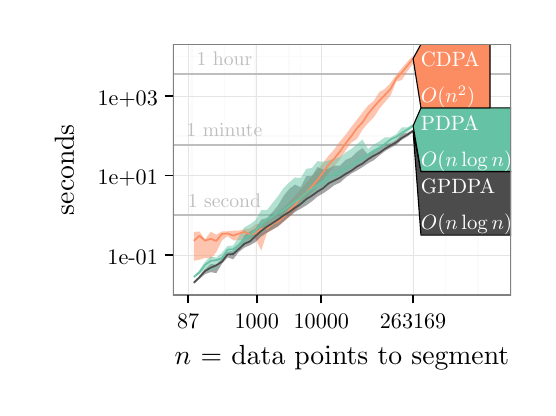
\begin{tikzpicture}[x=1pt,y=1pt]
\definecolor{fillColor}{RGB}{255,255,255}
\path[use as bounding box,fill=fillColor,fill opacity=0.00] (0,0) rectangle (180.67,130.09);
\begin{scope}
\path[clip] (  0.00,  0.00) rectangle (180.67,130.09);
\definecolor{drawColor}{RGB}{255,255,255}
\definecolor{fillColor}{RGB}{255,255,255}

\path[draw=drawColor,line width= 0.6pt,line join=round,line cap=round,fill=fillColor] (  0.00,  0.00) rectangle (180.68,130.09);
\end{scope}
\begin{scope}
\path[clip] ( 52.45, 33.48) rectangle (174.67,124.09);
\definecolor{fillColor}{RGB}{255,255,255}

\path[fill=fillColor] ( 52.45, 33.48) rectangle (174.67,124.09);
\definecolor{drawColor}{gray}{0.98}

\path[draw=drawColor,line width= 0.6pt,line join=round] ( 52.45, 33.60) --
	(174.67, 33.60);

\path[draw=drawColor,line width= 0.6pt,line join=round] ( 52.45, 62.29) --
	(174.67, 62.29);

\path[draw=drawColor,line width= 0.6pt,line join=round] ( 52.45, 90.99) --
	(174.67, 90.99);

\path[draw=drawColor,line width= 0.6pt,line join=round] ( 52.45,119.68) --
	(174.67,119.68);

\path[draw=drawColor,line width= 0.6pt,line join=round] ( 59.42, 33.48) --
	( 59.42,124.09);

\path[draw=drawColor,line width= 0.6pt,line join=round] ( 71.09, 33.48) --
	( 71.09,124.09);

\path[draw=drawColor,line width= 0.6pt,line join=round] ( 94.43, 33.48) --
	( 94.43,124.09);

\path[draw=drawColor,line width= 0.6pt,line join=round] ( 82.06, 33.48) --
	( 82.06,124.09);

\path[draw=drawColor,line width= 0.6pt,line join=round] ( 98.63, 33.48) --
	( 98.63,124.09);

\path[draw=drawColor,line width= 0.6pt,line join=round] (150.94, 33.48) --
	(150.94,124.09);

\path[draw=drawColor,line width= 0.6pt,line join=round] (162.61, 33.48) --
	(162.61,124.09);
\definecolor{drawColor}{gray}{0.90}

\path[draw=drawColor,line width= 0.2pt,line join=round] ( 52.45, 47.94) --
	(174.67, 47.94);

\path[draw=drawColor,line width= 0.2pt,line join=round] ( 52.45, 76.64) --
	(174.67, 76.64);

\path[draw=drawColor,line width= 0.2pt,line join=round] ( 52.45,105.34) --
	(174.67,105.34);

\path[draw=drawColor,line width= 0.2pt,line join=round] ( 82.76, 33.48) --
	( 82.76,124.09);

\path[draw=drawColor,line width= 0.2pt,line join=round] (106.11, 33.48) --
	(106.11,124.09);

\path[draw=drawColor,line width= 0.2pt,line join=round] ( 58.00, 33.48) --
	( 58.00,124.09);

\path[draw=drawColor,line width= 0.2pt,line join=round] (139.27, 33.48) --
	(139.27,124.09);
\definecolor{drawColor}{RGB}{190,190,190}

\path[draw=drawColor,line width= 0.6pt,line join=round] ( 52.45, 62.29) -- (174.67, 62.29);

\path[draw=drawColor,line width= 0.6pt,line join=round] ( 52.45, 87.80) -- (174.67, 87.80);

\path[draw=drawColor,line width= 0.6pt,line join=round] ( 52.45,113.32) -- (174.67,113.32);
\definecolor{fillColor}{RGB}{252,141,98}

\path[fill=fillColor,fill opacity=0.50] ( 60.03, 56.31) --
	( 62.07, 56.41) --
	( 64.10, 53.63) --
	( 66.13, 56.33) --
	( 68.16, 55.29) --
	( 70.19, 56.44) --
	( 72.22, 56.53) --
	( 74.26, 56.71) --
	( 76.29, 56.77) --
	( 78.32, 57.32) --
	( 80.35, 57.55) --
	( 82.38, 59.09) --
	( 84.41, 59.27) --
	( 86.44, 60.25) --
	( 88.48, 61.93) --
	( 90.51, 63.71) --
	( 92.54, 65.22) --
	( 94.57, 67.03) --
	( 96.60, 69.35) --
	( 98.63, 71.70) --
	(100.67, 73.89) --
	(102.70, 76.20) --
	(104.73, 78.62) --
	(106.76, 81.34) --
	(108.79, 83.90) --
	(110.82, 86.17) --
	(112.86, 89.06) --
	(114.89, 91.40) --
	(116.92, 94.17) --
	(118.95, 96.82) --
	(120.98, 99.43) --
	(123.01,101.96) --
	(125.04,103.61) --
	(127.08,106.85) --
	(129.11,108.01) --
	(131.14,110.14) --
	(133.17,113.05) --
	(135.20,115.46) --
	(137.23,117.84) --
	(139.27,119.97) --
	(139.27,117.05) --
	(137.23,114.38) --
	(135.20,111.17) --
	(133.17,110.63) --
	(131.14,105.59) --
	(129.11,103.24) --
	(127.08,100.79) --
	(125.04, 97.63) --
	(123.01, 95.66) --
	(120.98, 93.22) --
	(118.95, 89.83) --
	(116.92, 88.50) --
	(114.89, 85.63) --
	(112.86, 82.61) --
	(110.82, 80.12) --
	(108.79, 77.65) --
	(106.76, 75.15) --
	(104.73, 72.82) --
	(102.70, 70.51) --
	(100.67, 68.28) --
	( 98.63, 65.92) --
	( 96.60, 63.83) --
	( 94.57, 61.72) --
	( 92.54, 60.00) --
	( 90.51, 58.57) --
	( 88.48, 57.08) --
	( 86.44, 55.93) --
	( 84.41, 49.53) --
	( 82.38, 53.78) --
	( 80.35, 54.02) --
	( 78.32, 53.50) --
	( 76.29, 53.32) --
	( 74.26, 53.21) --
	( 72.22, 54.79) --
	( 70.19, 53.21) --
	( 68.16, 48.97) --
	( 66.13, 46.55) --
	( 64.10, 46.93) --
	( 62.07, 46.23) --
	( 60.03, 45.90) --
	cycle;
\definecolor{fillColor}{RGB}{77,77,77}

\path[fill=fillColor,fill opacity=0.50] ( 60.03, 38.22) --
	( 62.07, 40.44) --
	( 64.10, 42.83) --
	( 66.13, 44.66) --
	( 68.16, 44.55) --
	( 70.19, 46.78) --
	( 72.22, 49.08) --
	( 74.26, 49.48) --
	( 76.29, 51.50) --
	( 78.32, 54.93) --
	( 80.35, 56.41) --
	( 82.38, 57.59) --
	( 84.41, 60.70) --
	( 86.44, 61.34) --
	( 88.48, 63.44) --
	( 90.51, 65.92) --
	( 92.54, 69.35) --
	( 94.57, 71.84) --
	( 96.60, 73.37) --
	( 98.63, 72.43) --
	(100.67, 76.42) --
	(102.70, 76.52) --
	(104.73, 79.73) --
	(106.76, 78.79) --
	(108.79, 79.14) --
	(110.82, 80.25) --
	(112.86, 80.26) --
	(114.89, 82.28) --
	(116.92, 83.17) --
	(118.95, 85.16) --
	(120.98, 86.58) --
	(123.01, 84.11) --
	(125.04, 85.53) --
	(127.08, 86.82) --
	(129.11, 87.95) --
	(131.14, 88.45) --
	(133.17, 89.50) --
	(135.20, 91.81) --
	(137.23, 92.09) --
	(139.27, 93.26) --
	(139.27, 92.31) --
	(137.23, 90.78) --
	(135.20, 89.57) --
	(133.17, 87.77) --
	(131.14, 86.69) --
	(129.11, 85.47) --
	(127.08, 83.89) --
	(125.04, 82.17) --
	(123.01, 81.08) --
	(120.98, 79.71) --
	(118.95, 78.46) --
	(116.92, 77.38) --
	(114.89, 75.95) --
	(112.86, 74.09) --
	(110.82, 73.18) --
	(108.79, 71.62) --
	(106.76, 70.21) --
	(104.73, 69.05) --
	(102.70, 67.34) --
	(100.67, 65.88) --
	( 98.63, 64.65) --
	( 96.60, 63.48) --
	( 94.57, 61.86) --
	( 92.54, 60.13) --
	( 90.51, 58.25) --
	( 88.48, 57.19) --
	( 86.44, 55.98) --
	( 84.41, 54.64) --
	( 82.38, 52.66) --
	( 80.35, 51.50) --
	( 78.32, 50.63) --
	( 76.29, 49.03) --
	( 74.26, 46.40) --
	( 72.22, 47.08) --
	( 70.19, 44.76) --
	( 68.16, 41.40) --
	( 66.13, 41.75) --
	( 64.10, 41.04) --
	( 62.07, 39.31) --
	( 60.03, 37.60) --
	cycle;
\definecolor{fillColor}{RGB}{102,194,165}

\path[fill=fillColor,fill opacity=0.50] ( 60.03, 40.23) --
	( 62.07, 42.54) --
	( 64.10, 45.54) --
	( 66.13, 47.36) --
	( 68.16, 47.00) --
	( 70.19, 48.76) --
	( 72.22, 51.21) --
	( 74.26, 51.39) --
	( 76.29, 54.47) --
	( 78.32, 57.95) --
	( 80.35, 59.09) --
	( 82.38, 60.55) --
	( 84.41, 64.19) --
	( 86.44, 64.13) --
	( 88.48, 66.73) --
	( 90.51, 69.29) --
	( 92.54, 72.23) --
	( 94.57, 74.19) --
	( 96.60, 75.98) --
	( 98.63, 75.75) --
	(100.67, 79.06) --
	(102.70, 79.38) --
	(104.73, 81.85) --
	(106.76, 81.61) --
	(108.79, 82.09) --
	(110.82, 82.89) --
	(112.86, 83.27) --
	(114.89, 84.96) --
	(116.92, 86.27) --
	(118.95, 87.91) --
	(120.98, 89.65) --
	(123.01, 86.27) --
	(125.04, 87.83) --
	(127.08, 89.02) --
	(129.11, 90.45) --
	(131.14, 90.47) --
	(133.17, 91.61) --
	(135.20, 94.03) --
	(137.23, 94.05) --
	(139.27, 95.26) --
	(139.27, 94.21) --
	(137.23, 92.46) --
	(135.20, 91.15) --
	(133.17, 89.18) --
	(131.14, 88.33) --
	(129.11, 87.05) --
	(127.08, 85.70) --
	(125.04, 83.73) --
	(123.01, 82.47) --
	(120.98, 81.40) --
	(118.95, 80.04) --
	(116.92, 79.04) --
	(114.89, 77.51) --
	(112.86, 75.46) --
	(110.82, 74.73) --
	(108.79, 73.12) --
	(106.76, 71.77) --
	(104.73, 70.33) --
	(102.70, 69.10) --
	(100.67, 67.11) --
	( 98.63, 65.96) --
	( 96.60, 64.97) --
	( 94.57, 63.04) --
	( 92.54, 61.79) --
	( 90.51, 59.65) --
	( 88.48, 58.43) --
	( 86.44, 57.03) --
	( 84.41, 55.96) --
	( 82.38, 54.27) --
	( 80.35, 53.42) --
	( 78.32, 51.39) --
	( 76.29, 50.63) --
	( 74.26, 48.07) --
	( 72.22, 48.13) --
	( 70.19, 46.40) --
	( 68.16, 42.83) --
	( 66.13, 42.08) --
	( 64.10, 42.83) --
	( 62.07, 41.04) --
	( 60.03, 39.78) --
	cycle;
\definecolor{drawColor}{RGB}{252,141,98}

\path[draw=drawColor,line width= 0.6pt,line join=round] ( 60.03, 53.07) --
	( 62.07, 54.88) --
	( 64.10, 53.13) --
	( 66.13, 53.78) --
	( 68.16, 53.02) --
	( 70.19, 55.57) --
	( 72.22, 55.72) --
	( 74.26, 54.95) --
	( 76.29, 55.62) --
	( 78.32, 56.36) --
	( 80.35, 55.24) --
	( 82.38, 55.87) --
	( 84.41, 57.41) --
	( 86.44, 57.49) --
	( 88.48, 59.16) --
	( 90.51, 60.08) --
	( 92.54, 61.78) --
	( 94.57, 64.16) --
	( 96.60, 66.01) --
	( 98.63, 68.66) --
	(100.67, 70.54) --
	(102.70, 72.71) --
	(104.73, 75.08) --
	(106.76, 77.81) --
	(108.79, 80.75) --
	(110.82, 82.83) --
	(112.86, 85.37) --
	(114.89, 88.25) --
	(116.92, 90.88) --
	(118.95, 93.69) --
	(120.98, 95.87) --
	(123.01, 98.97) --
	(125.04,101.44) --
	(127.08,103.68) --
	(129.11,105.79) --
	(131.14,108.00) --
	(133.17,111.70) --
	(135.20,113.91) --
	(137.23,116.37) --
	(139.27,118.90);
\definecolor{drawColor}{gray}{0.30}

\path[draw=drawColor,line width= 0.6pt,line join=round] ( 60.03, 37.91) --
	( 62.07, 39.90) --
	( 64.10, 42.16) --
	( 66.13, 43.37) --
	( 68.16, 44.22) --
	( 70.19, 45.49) --
	( 72.22, 48.16) --
	( 74.26, 48.31) --
	( 76.29, 50.08) --
	( 78.32, 52.01) --
	( 80.35, 52.88) --
	( 82.38, 54.84) --
	( 84.41, 56.64) --
	( 86.44, 58.16) --
	( 88.48, 59.46) --
	( 90.51, 60.80) --
	( 92.54, 62.26) --
	( 94.57, 63.52) --
	( 96.60, 65.03) --
	( 98.63, 66.36) --
	(100.67, 68.12) --
	(102.70, 69.37) --
	(104.73, 70.86) --
	(106.76, 72.08) --
	(108.79, 73.87) --
	(110.82, 74.89) --
	(112.86, 75.91) --
	(114.89, 77.25) --
	(116.92, 78.37) --
	(118.95, 79.89) --
	(120.98, 80.98) --
	(123.01, 82.57) --
	(125.04, 83.82) --
	(127.08, 84.85) --
	(129.11, 86.34) --
	(131.14, 87.50) --
	(133.17, 88.67) --
	(135.20, 90.26) --
	(137.23, 91.44) --
	(139.27, 92.78);
\definecolor{drawColor}{RGB}{102,194,165}

\path[draw=drawColor,line width= 0.6pt,line join=round] ( 60.03, 40.01) --
	( 62.07, 41.66) --
	( 64.10, 44.39) --
	( 66.13, 45.81) --
	( 68.16, 46.07) --
	( 70.19, 46.82) --
	( 72.22, 49.86) --
	( 74.26, 50.04) --
	( 76.29, 51.67) --
	( 78.32, 53.83) --
	( 80.35, 55.06) --
	( 82.38, 56.95) --
	( 84.41, 59.02) --
	( 86.44, 60.66) --
	( 88.48, 61.85) --
	( 90.51, 63.17) --
	( 92.54, 64.32) --
	( 94.57, 65.76) --
	( 96.60, 67.22) --
	( 98.63, 68.54) --
	(100.67, 70.45) --
	(102.70, 71.88) --
	(104.73, 73.31) --
	(106.76, 74.39) --
	(108.79, 76.12) --
	(110.82, 77.09) --
	(112.86, 77.91) --
	(114.89, 79.28) --
	(116.92, 80.29) --
	(118.95, 81.85) --
	(120.98, 82.92) --
	(123.01, 84.31) --
	(125.04, 85.66) --
	(127.08, 86.72) --
	(129.11, 88.11) --
	(131.14, 89.70) --
	(133.17, 90.62) --
	(135.20, 92.08) --
	(137.23, 93.31) --
	(139.27, 94.60);
\definecolor{drawColor}{RGB}{190,190,190}

\node[text=drawColor,anchor=base,inner sep=0pt, outer sep=0pt, scale=  0.71] at ( 71.09, 65.23) {1 second};

\node[text=drawColor,anchor=base,inner sep=0pt, outer sep=0pt, scale=  0.71] at ( 71.09, 90.74) {1 minute};

\node[text=drawColor,anchor=base,inner sep=0pt, outer sep=0pt, scale=  0.71] at ( 71.09,116.26) {1 hour};
\end{scope}
\begin{scope}
\path[clip] ( 52.45, 33.48) rectangle (174.67,124.09);
\definecolor{drawColor}{RGB}{0,0,0}
\definecolor{fillColor}{gray}{0.30}

\path[draw=drawColor,line width= 0.4pt,line join=round,line cap=round,fill=fillColor] (139.27, 92.78) --
	(142.11, 78.11) --
	(180.67, 78.11) --
	(180.67, 55.12) --
	(142.11, 55.12) --
	cycle;
\definecolor{fillColor}{RGB}{102,194,165}

\path[draw=drawColor,line width= 0.4pt,line join=round,line cap=round,fill=fillColor] (139.27, 94.60) --
	(142.11,101.10) --
	(180.67,101.10) --
	(180.67, 78.11) --
	(142.11, 78.11) --
	cycle;
\definecolor{fillColor}{RGB}{252,141,98}

\path[draw=drawColor,line width= 0.4pt,line join=round,line cap=round,fill=fillColor] (139.27,118.90) --
	(142.11,124.09) --
	(167.07,124.09) --
	(167.07,101.10) --
	(142.11,101.10) --
	cycle;
\definecolor{drawColor}{RGB}{255,255,255}

\node[text=drawColor,anchor=base west,inner sep=0pt, outer sep=0pt, scale=  0.75] at (142.11, 69.99) {GPDPA};

\node[text=drawColor,anchor=base west,inner sep=0pt, outer sep=0pt, scale=  0.75] at (142.11, 57.03) {$O(n \log n)$};

\node[text=drawColor,anchor=base west,inner sep=0pt, outer sep=0pt, scale=  0.75] at (142.11, 92.98) {PDPA};

\node[text=drawColor,anchor=base west,inner sep=0pt, outer sep=0pt, scale=  0.75] at (142.11, 80.02) {$O(n \log n)$};

\node[text=drawColor,anchor=base west,inner sep=0pt, outer sep=0pt, scale=  0.75] at (142.11,115.97) {CDPA};

\node[text=drawColor,anchor=base west,inner sep=0pt, outer sep=0pt, scale=  0.75] at (142.11,103.01) {$O(n^2)$};
\definecolor{drawColor}{gray}{0.50}

\path[draw=drawColor,line width= 0.6pt,line join=round,line cap=round] ( 52.45, 33.48) rectangle (174.67,124.09);
\end{scope}
\begin{scope}
\path[clip] (  0.00,  0.00) rectangle (180.67,130.09);
\definecolor{drawColor}{RGB}{0,0,0}

\node[text=drawColor,anchor=base east,inner sep=0pt, outer sep=0pt, scale=  0.80] at ( 47.05, 44.64) {1e-01};

\node[text=drawColor,anchor=base east,inner sep=0pt, outer sep=0pt, scale=  0.80] at ( 47.05, 73.33) {1e+01};

\node[text=drawColor,anchor=base east,inner sep=0pt, outer sep=0pt, scale=  0.80] at ( 47.05,102.03) {1e+03};
\end{scope}
\begin{scope}
\path[clip] (  0.00,  0.00) rectangle (180.67,130.09);
\definecolor{drawColor}{RGB}{0,0,0}

\path[draw=drawColor,line width= 0.6pt,line join=round] ( 49.45, 47.94) --
	( 52.45, 47.94);

\path[draw=drawColor,line width= 0.6pt,line join=round] ( 49.45, 76.64) --
	( 52.45, 76.64);

\path[draw=drawColor,line width= 0.6pt,line join=round] ( 49.45,105.34) --
	( 52.45,105.34);
\end{scope}
\begin{scope}
\path[clip] (  0.00,  0.00) rectangle (180.67,130.09);
\definecolor{drawColor}{RGB}{0,0,0}

\path[draw=drawColor,line width= 0.6pt,line join=round] ( 82.76, 30.48) --
	( 82.76, 33.48);

\path[draw=drawColor,line width= 0.6pt,line join=round] (106.11, 30.48) --
	(106.11, 33.48);

\path[draw=drawColor,line width= 0.6pt,line join=round] ( 58.00, 30.48) --
	( 58.00, 33.48);

\path[draw=drawColor,line width= 0.6pt,line join=round] (139.27, 30.48) --
	(139.27, 33.48);
\end{scope}
\begin{scope}
\path[clip] (  0.00,  0.00) rectangle (180.67,130.09);
\definecolor{drawColor}{RGB}{0,0,0}

\node[text=drawColor,anchor=base,inner sep=0pt, outer sep=0pt, scale=  0.80] at ( 82.76, 21.46) {1000};

\node[text=drawColor,anchor=base,inner sep=0pt, outer sep=0pt, scale=  0.80] at (106.11, 21.46) {10000};

\node[text=drawColor,anchor=base,inner sep=0pt, outer sep=0pt, scale=  0.80] at ( 58.00, 21.46) {87};

\node[text=drawColor,anchor=base,inner sep=0pt, outer sep=0pt, scale=  0.80] at (139.27, 21.46) {263169};
\end{scope}
\begin{scope}
\path[clip] (  0.00,  0.00) rectangle (180.67,130.09);
\definecolor{drawColor}{RGB}{0,0,0}

\node[text=drawColor,anchor=base,inner sep=0pt, outer sep=0pt, scale=  1.00] at (113.56,  8.40) {$n$ = data points to segment};
\end{scope}
\begin{scope}
\path[clip] (  0.00,  0.00) rectangle (180.67,130.09);
\definecolor{drawColor}{RGB}{0,0,0}

\node[text=drawColor,rotate= 90.00,anchor=base,inner sep=0pt, outer sep=0pt, scale=  1.00] at ( 16.66, 78.78) {seconds};
\end{scope}
\end{tikzpicture}
